\documentclass[number=03]{assignment}
\title{Design with Microcontrollers \& Computer architecture}
\chead{Assignment 01}
\rhead{ALU design}
%\date{February - June 2020}

\newif\ifanswers
\answerstrue % comment out to hide answers

\newcommand{\deadline}{23:59 hours on Friday November 19th 2021}

\newcommand{\alupkgfile}{\colorfilename{alu\_pkg.sv}}
\newcommand{\alusvfile}{\colorfilename{alu.sv}}
\newcommand{\alutbfile}{\colorfilename{tb\_alu.sv}}

% Begin document
\begin{document}

\setcounter{chapter}{1}
\chapter*{Assignment 01 \\ \acs{ALU} design}
\acresetall
% ======================================
% Objective
% ======================================
\section{Objectives}
\begin{itemize}
\item To understand the basic concept of an \ac{ALU}.
\item To design and simulate an \ac{ALU}.
\item To understand how the \ac{ALU} provides a status of the result of each operation. 
\end{itemize}

% ======================================
% Deadline
% ======================================
\section{Deadline}
\alertblue{\deadline}.
% ======================================
% Teamwork policy
% ======================================
\section{Teamwork policy}
This is an individual assignment. 
% % ======================================
% % Pre-requisites
% % ======================================
% \section{Pre-requisites}
% It is assumed that you are familiar with working with \ModelSim and \Quartus. 
% If you require assistance, you can refer to the first assignment tutorial.
% ======================================
% Background
% ======================================
\section{Background}\label{Sec:Background}
An \acf{ALU} combines a variety of both mathematical, boolean, and logical operations into a single unit.
The schematic symbol of an \ac{ALU} is shown in \fref{Figure:ALU}.

  %
  % Figure ALU
  %
 \begin{figure}[!htb]
  \centering
  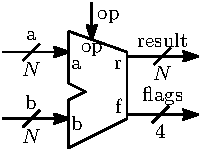
\includegraphics[scale=1.4]{ALU_flags}
  \caption{\ac{ALU} symbol.}
  \label{Figure:ALU}
\end{figure} 
  %
  % End Figure ALU
  %
  
In \fref{Figure:ALU}, the \ac{ALU} receives two $N$-bit operands, \code{a} and \code{b}, as well as a control signal \code{op}, which indicates the type of operation the \ac{ALU} must perform. 
More specifically, the value of \code{op} specifies whether the \ac{ALU} should perform an addition, a subtraction or any bitwise logical operation between the two input operands.
The \ac{ALU} delivers an $N$-bit output, labelled as \code{result} in \fref{Figure:ALU}, which corresponds to the result of the arithmetic or logical operation.
In addition to this, the \ac{ALU} delivers a 4-bit output, labelled as \code{flags} in \fref{Figure:ALU}, which provides a status regarding the result of each \ac{ALU} operation.
More specifically, the output \code{flags} indicates whether the output \code{result} is zero or negative, as well as whether an arithmetic operation produced an overflow or a carry out condition.
  
%
\begin{table}[!htb]
\centering
\caption{\acs{ALU} ports.}
\label{Table:ALU_ports}
\begin{threeparttable}
\begin{tabular}{l|l|l}
\hline\hline
Port name & Direction & Description \\
\hline\hline
\code{a}          & \code{input}  & Operand a. \\ \hline
\code{b}          & \code{input}  & Operand b. \\ \hline  
\code{op}         & \code{input}  & Operation to be performed. \\ \hline  
\code{result}     & \code{output} & Result from the arithmetic or logical operation.\\ \hline 
\code{z}          & \code{output} & Zero flag. Active high when result is exactly zero.\\ \hline
\code{n}          & \code{output} & Negative flag. Active high when result is negative. \\ \hline
\multirow{2}{*}{\code{v}}          & \multirow{2}{*}{\code{output}} & Overflow. Active high when an overflow occurs in an\\
 & & arithmetic operation. \\ \hline
 \multirow{2}{*}{\code{c}}          & \multirow{2}{*}{\code{output}} & Carry flag. Active high when a carry out is produced in an \\
 & & arithmetic operation. \\ \hline
\hline
\end{tabular}
\end{threeparttable}
\end{table}
%

Note that the output \code{flags} of \fref{Figure:ALU} is split into outputs \code{z}, \code{n}, \code{v}, and \code{c} in \tref{Table:ALU_ports}.


%The operations that the \ac{ALU} must perform are described in \tref{Table:ALU_operations}.

%%
%\begin{table}[!htb]
%\centering
%\caption{\acs{ALU} operations.}
%\label{Table:ALU_operations}
%\begin{tabular}{l|l|l}
%\hline\hline
% Operation type & Enum name & Meaning \\
% \hline\hline
% \multirow{2}{*}{Arithmetic} & \code{ALU\_ADD} & Addition    \\
%                             & \code{ALU\_SUB} & Subtraction \\
%                                                         \hline
% \multirow{6}{*}{Logical} & \code{ALU\_NAND} & Logical NAND \\
%                          & \code{ALU\_NOR}  & Logical NOR  \\
%                          & \code{ALU\_XNOR} & Logical XNOR \\
%                          & \code{ALU\_AND} & Logical AND   \\
%                          & \code{ALU\_OR}  & Logical OR    \\
%                          & \code{ALU\_XOR} & Logical XOR   \\
%                          \hline
% \multirow{4}{*}{Shift} & \code{ALU\_SLL} & Shift left logical \\
%                             & \code{ALU\_SRL} & Shift right logical \\
%                             & \code{ALU\_SLA} & Shift left arithmetic \\
%                             & \code{ALU\_SRA} & Shift right arithmetic \\
%                             \hline
% \multirow{2}{*}{Load with immediate} & \code{ALU\_LUI} & Load upper with immediate \\
%                                      & \code{ALU\_LLI} & Load lower with immediate  \\
%                             \hline
%Comparison & \code{ALU\_CMP} & Compares \code{a} and \code{b} \\ 
% \hline\hline
% \end{tabular}
%\end{table}
%%


%These operations must be defined in a user-defined \enum data type named \code{alu\_op\_t} and declared in a ??
%Moreover, \tref{Table:ALU_operations} specifies the name of the \enum you must use for the different \ac{ALU} operations.

 
\newpage

% ======================================
% ISA and uA
% ====================================== 
\newpage
\section{ALU design exercise}\label{Sec:ALU_design}
In this assignment, you are required to design and simulate an \ac{ALU}.
In order to allow flexibility in this assignment, you may choose to design your \ac{ALU} using either Logisim simulator or \SV \ac{HDL}.
You are required to submit \alertblue{ONLY ONE} \ac{ALU} design.
More specifically, you might submit the design using Logisim \alertblue{OR} \SV.

\alertred{IMPORTANT!}
Please note that \SV is not covered as a topic in this course.
Hence, the \ac{ALU} design with \SV is completely optional.
However, this challenge might be a great opportunity to learn a sought-after industry skill, if you are interested in pursuing a career in the design and verification of \acp{IC}.

\sref{Sec:ALU_Logisim} and \sref{Sec:ALU_SV} describe the design specifications for designing the \ac{ALU} in Logisim and \SV, respectively.

\subsection{ALU design in Logisim}\label{Sec:ALU_Logisim}
The \ac{ALU} designed using Logisim must be a 4-bit \ac{ALU} with flags generation.
The input and output ports of the \ac{ALU} are specified in the list below.
\begin{itemize}
\item Two 4-bit inputs, namely \codeblue{a} and \codeblue{b}. 
These inputs are the operands of the \ac{ALU}.
\item Input \codeblue{op}, which will be used by the \ac{ALU} in order to select which operation will be performed.
Note that the number of bits for the input \codeblue{op} must be selected according to the number of operation supported by the \ac{ALU}. 
It is your task to determine the number of bits for \codeblue{op}.
\item 4-bit output \codeblue{result}.
This output contains the result of the arithmetic or logical operation.
\item Output port \codeblue{z}. Zero flag.
\item Output port \codeblue{n}. Negative flag.
\item Output port \codeblue{v}. Overflow flag. 
This flag should only be enabled when the \ac{ALU} performs an arithmetic operation. 
For logical operations, this flag should always be 0.
\item Output port \codeblue{c}. Carry flag.
This flag should only be enabled when the \ac{ALU} performs an arithmetic operation. 
For logical operations, this flag should always be 0.
 
\end{itemize}



\subsection{ALU design in SystemVerilog}\label{Sec:ALU_SV}

\subsubsection{Previous work}
If you opt for designing and simulating the \ac{ALU} in \SV, I strongly suggest that you to complete the \SV tutorial that is included with this assignment.
After completing the tutorial, you might come back to complete the rest of this section.

\subsubsection{ALU design exercise}
You are provide with \alupkgfile, \alusvfile, and \alutbfile \SV files.
Each of these files is explained below.
\begin{itemize}
\item \alupkgfile contains a basic definition of the \ac{ALU} operations.
\SV package files are somewhat analogous to \code{.h} header files in C language.
\SV package files are useful to declare and share parameters and user-defined data types among several \SV files and modules that are included in a single design.
For this assignment, you are not required to modify \alupkgfile.
\item \alusvfile contains a basic skeleton of an \ac{ALU} design.
However, this file is incomplete and you are required to include \SV code for completing the \ac{ALU} design.
More specifically, you are required to complete the \SV code that will perform each of the \ac{ALU} operations, as well as the logic required for generating the \ac{ALU} flags \codeblue{z}, \codeblue{n}, \codeblue{v}, and \codeblue{c}.
\item \alutbfile is a testbench file for the \ac{ALU} module declared in \alusvfile. 
More specifically, \alutbfile generates stimuli and basic functionality tests for the \ac{ALU} input ports, to which the \ac{ALU} must respond correctly.
This file instantiates (uses) one copy of the \ac{ALU} design and connects its ports to signals declared in the testbench. 
You are not required to modify this file. 
However, you are encouraged to have a look at it and understand the code provided.
You are also encouraged to modify this file, in order to apply different test scenarios, \textbf{after} you have completed this assignment.
\end{itemize} 

\subsubsection{ALU simulation in ModelSim}
In order to verify the correct operation of your \ac{ALU}, you are required to perform a simulation using ModelSim.
For this purpose, you might follow the steps provided in the tutorial files for compiling and simulating your design.
When working with \SV packages, it is recommended to specify the order in which the \SV files will be compiled.
More specifically, in \ModelSim, you should select  \textbf{Compile} $\rightarrow$ \textbf{Compile order}, and make sure that \alupkgfile is the first file in the list.

After successfully compiling all your \SV files, you might begin the simulation, as stated in the tutorial.
This include the steps necessary for adding and viewing waveforms into the simulation.
Note that once you have waveforms available in your simulation, you can change the radix (format) in which the signals are displayed. 
This is particularly useful when working with multi-bit width signals, such as the \ac{ALU} operands. 
For example, right-click on the input signal \code{a} in the \textbf{Wave} pane and select \textbf{Radix} $\rightarrow$ \textbf{Decimal}.

\subsubsection{ALU synthesis in Quartus}
\Quartus might be used for performing logic synthesis of the \ac{ALU}.
Synthesis is the process of generating logic gates from \SV (or any \ac{HDL}).
In other words, a synthesizer, such as \Quartus, will translate your \SV file into simple logic gates that will be later used for implementing the design in a \ac{FPGA} or an \ac{ASIC}.
\alertred{A design that can not be synthesized is a useless design.}
Use the tutorial as a reference in order to synthesize and observe the equivalent \ac{RTL} view of the \ac{ALU} using \Quartus.
Note that \Quartus must only be used to synthesize design units.
Testbenches are never synthesized.

\newpage
\section{Deliverables and submission instructions}\label{Sec:Deliverables}
This section details the deliverable and submission instructions for this assignment.

\subsection{Deliverables}
Please follow the delivery instructions below depending on your choice of \ac{ALU} design.
Remember that you are required to submit \alertblue{ONLY ONE} \ac{ALU} design, either in Logisim or \SV.

\subsubsection{ALU in Logisim}
Submit your \ac{ALU} \code{.circ} Logisim file. 

\subsubsection{ALU in \SV}
Submit the following items.
\begin{itemize}
\item \alusvfile. This file should contain the \ac{ALU} module definition and operation.
\item A screenshot of your \ModelSim simulation.
\item A screenshot of the \ac{ALU}'s \ac{RTL} view after synthesis in \Quartus.
\end{itemize}

\subsection{Submission}
Submit your assignment through Canvas \alertred{no later} than \deadline. 
\\

\alertblue{IMPORTANT!} This is a desing exercide.Therefore, there may be \alertviolet{multiple} correct answers.
\\

Please send any questions to \href{mailto:isaac.perez.andrade@tec.mx}{isaac.perez.andrade@tec.mx}.
\end{document}
s